\documentclass[a4paper,10pt]{article}
\usepackage{amsmath}
\usepackage{amsthm}
\newtheorem{mydef}{Definition}
\usepackage{url, hyperref}
\usepackage{amsthm}
\usepackage{amsfonts}
\usepackage{amssymb}
\newtheorem{theorem}{Theorem}
\newtheorem{lemma}{Lemma}
\usepackage{fullpage}
\usepackage{tikz}
\usepackage{float}
\usepackage{listings}
\usepackage{color}
\usepackage{mathtools}
\usepackage[T1]{fontenc}
\usepackage{subfigure}
\usepackage{algorithm}
\usepackage{algpseudocode}
\bibliographystyle{plain}


\title{Honors Project: Efficient segmentation algorithms for shark fin
identification}
\author{L. Cilli\'{e}, 16010450}
\date{October 18, 2013}

\begin{document}
\maketitle

\newpage
\tableofcontents

\newpage
\section{Introduction and background}
\subsection{}
Just as humans are identified by their fingerprints, sharks have an unique
dorsal fin structure.  Identifying shark sightings these days can be very
valuable.  In order to do that and also to match shark sightings, photos of
shark fins, as will be shown in the proposal, will be analysed by a computer. 
This will consist of comparing the edges in the image and segmenting the
foreground, the shark fin being most prominent,  from the background, the sea. 
Although the photos provided are of a good quality and only include the fin, the
foreground and background properties can still vary significantly, making this a
non-trivial problem.  This project aims to investigate efficient segmentation
algorithms for shark fin identification.  The approach will consist of
evaluating (by means of a computer) different methods for classifying foreground
and background, as well as segmenting the foreground successfully.  By doing so,
the burden on biological researchers can be reduced. 

\begin{figure}[H]
\centering
\mbox{\subfigure[Shark fin 1]{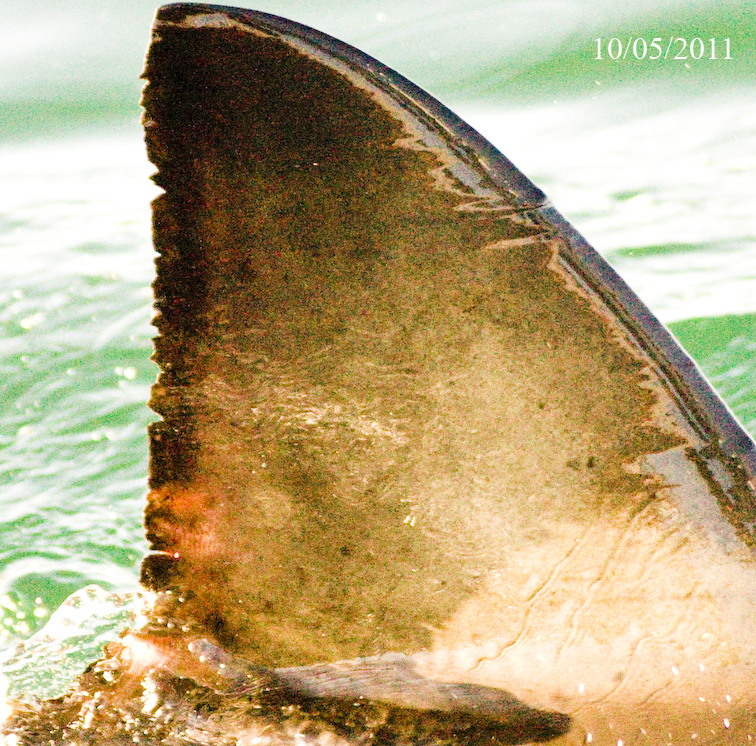
\includegraphics[width=1in]{haai1.jpg}} \quad
\subfigure[Shark fin 2]{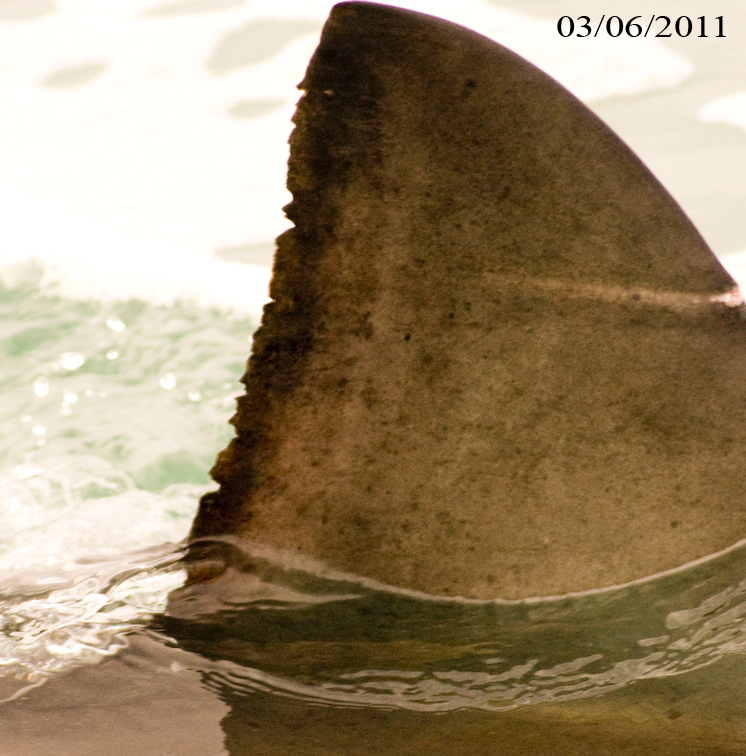
\includegraphics[width=1in]{haai2.jpg}}}
\caption{Examples of shark fin images}
\end{figure}


\subsection{}
Image segmentation is well known in the field of image processing.  It consists
of partitioning a digital image into multiple segments for some or other reason.
 Usually to make the image easier to analyse.  In other words each pixel is
assigned a label and all the pixels with the same label share a certain
property.  Image segmentation is typically used to locate an object or
boundaries in an image.  Well known examples where image processing are used is
in medical imaging to locate tumours for example, face and
fingerprint recognition and video surveillance.


\section{}


\section{Segmentation Algorithms}
\subsection{What is a cellular automaton?}
A cellular automaton consists of a grid of cells, where each one of the cells
can be in a finite number of states, say on and off.  This must be specified
beforehand.  Around each cell, a set of cells, called the cell's neighbourhood,
is defined.  An initial state, at time t = 0, is also assigned to each cell.  A
new generation of cells is then created according to a fixed rule or
mathematical function that determines the new state of the cell, by looking at
the current state of the cell as well as that of its neighbourhood.  This rule
is then applied to all of the cells simultaneously.  In this way, the cell's
state gets updated.  Note that the rules for each cell are the same and do not
change over time.  Two of the most common neighbourhood systems used are the Von
Neumann neighbourhood and the Moore neighbourhood which are shown below. 
Probably the most well-known example of a two dimensional automaton is Conway's
Game of Life.  See \cite{gol} for further details.

\begin{figure}[H]
\centering
\mbox{\subfigure{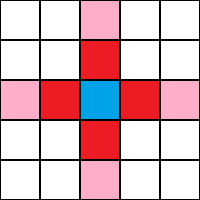
\includegraphics[width=1in]{VonNeumann.png}} \quad
\subfigure{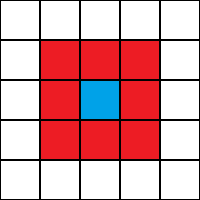
\includegraphics[width=1in]{Moore.png}}} \caption{Von Neumann and
Moore neighbourhood systems \cite{n}}
\end{figure}

\subsection{Growcut}
The Grow Cut algorithm is an interactive, multi-label segmentation algorithm for N-dimensional images.  The algorithm is based on cellular automata, i.e.,  the user labels a few pixels
and the rest of the image is then segmented automatically by a cellular automaton.  A cellular automaton consists of a grid of cells, where each one of the cells can be in 
a finite number of states, say on and off.   Around each cell, a set of cells, called the cell's neighbourhood is defined.  An initial state, at time $t = 0$, is also assigned to each cell.
A new generation of cells is then created according to a fixed rule or mathematical function that determines the new state of the cell, by looking at the current state of the cell as well
as that of its neighbourhood.  It is known that the same rules apply to each cell and do not change over time.
The algorithm is interactive, since the user can observe the segmentation and guide the algorithm in places where the segmentation is difficult to compute.
Some of the favourable properties of this algorithm is that it can do segmentation on complex images and that it works with images of any dimension. \\


\noindent The basic method on which the algorithm relies is the following.  A cellular automaton is an algorithm which is discrete in both space and time and operates on a 
lattice of pixels $p \in P \subset Z^{n}$.  A cellular automaton can be considered as a triplet, $A = (S, N, \delta)$, where $S$ is a set containing different states, $N$ is the
neighbourhood system of the cell and $\delta: S^{N} \rightarrow S $ is a transition rule.  This is the function which defines  the rule calculating the cell's state at time $t + 1$, given the states 
of the cell's neighbourhood at time $t$.  Two well known neighbourhood systems are the von Neumann and Moore neighbourhood systems.  The cell state referred to is also
considered a triplet $(l_{p}, \theta_{p}, \overrightarrow{C}_{p})$, where $l_{p}$ is the label of the cell($K$ labels in total), $\theta_{p}$ is the 'strength' of the cell and $\overrightarrow{C}_{p}$ is
the cell feature vector.  Without loss of generality it can be assumed that $\theta_{p} \in [0,1]$. 

The initial state of the pixels is set to $l_{p} = 0, \theta_{p} = 0, \overrightarrow{C}_{p} = RGB_{p}$, where $RGB_{p}$ is a three dimensional vector of the pixel's colour in 
the RGB space.  The goal of the segmentation is to assign one of the possible $K$ labels to each one of the pixels.  The user starts the segmentation by marking specific pixels as
foreground and others as background.  This sets the initial state of each pixel.  While the labels are being updated, the user can correct and guide the process if desired.  \\

\newpage
\noindent The pseudo code for the automata evolution rule is shown below. 
\begin{algorithm}[H]
\begin{algorithmic}[1]
 \State // For each cell...
 \For{$\forall p \in P$}
 \State // Copy previous state
 \State $l^{t+1}_{p} = l^{t}_{p}$;
 \State $\theta_{p}^{t+1} = \theta_{p}^{t}$;
 \State // Neighbours try to attack the current cell
 \For{$\forall q \in N(p)$}
 \If{$g(\| \overrightarrow{C}_{p} - \overrightarrow{C}_{q} \|_{2}) \cdot \theta^{t}_{q} > \theta_{p}^{t}$}
 \State $l^{t+1}_{p} = l^{t}_{q}$
 \State $\theta^{t+1}_{p} = g(\| \overrightarrow{C}_{p} - \overrightarrow{C}_{q} \|_{2}) \cdot \theta^{t}_{q}$
 \EndIf
 \EndFor
 \EndFor
\end{algorithmic}
\end{algorithm}

\noindent where $g$ is a monotonous decreasing function bounded to $[0, 1]$.  The function is given by
\[
g(x) = 1 - \frac{x}{max\| \overrightarrow{C} \|_{2}}. 
\]


\noindent The algorithm has been modified in the following way.  One of the main features that needed attention was the damping function $g$.  
By changing the exponent of the term $\frac{x}{max\| \overrightarrow{C} \|_{2}}$ to $\frac{3}{2}$, thus $\left ({\frac{x}{max\| \overrightarrow{C} \|_{2}}}\right ) ^\frac{3}{2}$,
an immediate result was seen.  The algorithm acted much more accurately around the edges.  Next, the 'defend strength' of each pixel was modified also by playing with exponents
of certain parts of the code.  A sobel filter was used in detecting the edges.  A sobel filter calculates the gradient of the intensity of each pixel, giving the direction of the largest possible increase from light to dark and also the rate of change in that specific direction.   This results in showing how abruptly or smoothly the images changes at that point and then how likely it is that that part represents an edge.  The figure below shows a sobel filter acting on a shark fin image.  The edges of the shark fin can clearly be seen.  The main purpose of these changes was to improve accuracy when detecting the edges.
\\
\begin{figure}[H]
 \centering
 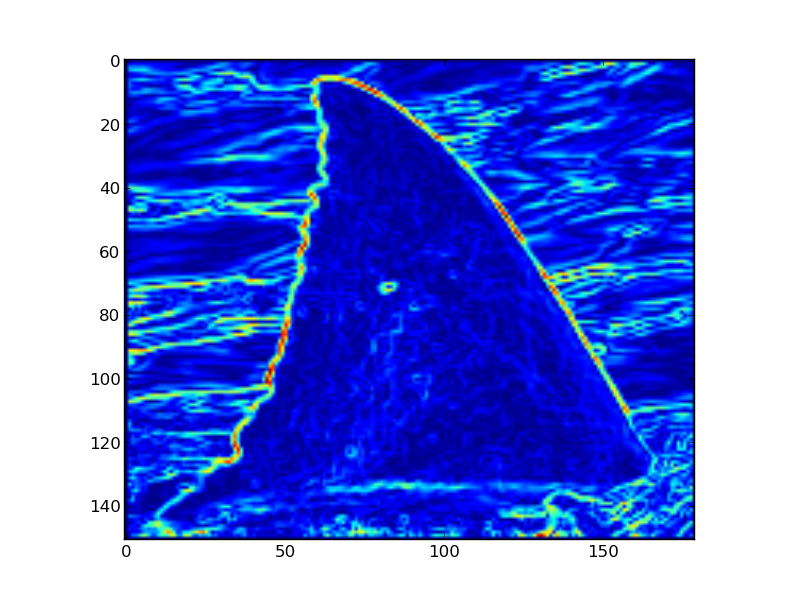
\includegraphics[width=2.5in, height=2in]{haais}
 \caption{A sobel filter applied to a shark fin image}
 \label{fin1}
\end{figure}

\newpage
\noindent Here is a comparison between the effect of the original algorithm on one of the shark fin images and the effect of the modified version of the algorithm on the same image.
\begin{figure}[H]
 \centering
 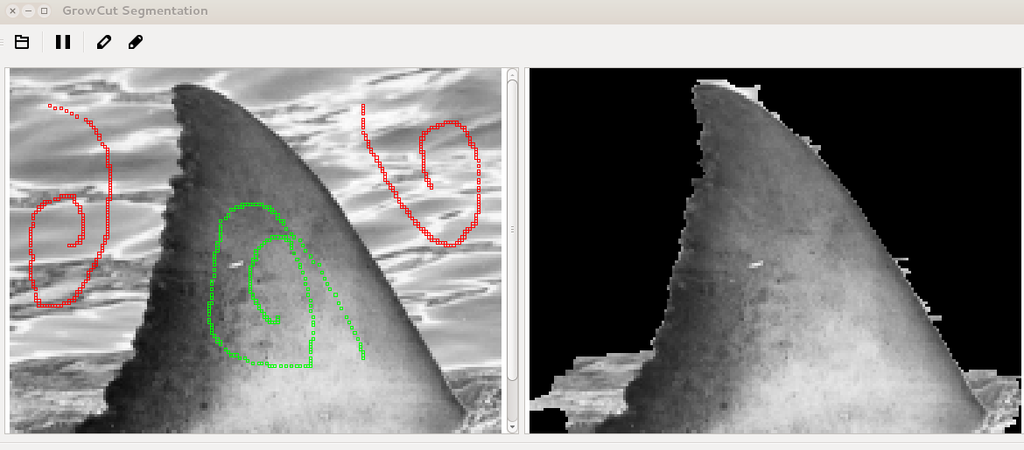
\includegraphics[width=4in, height=1.8in]{haaio}
 \caption{The effect of the original algorithm}
 \label{fin1}
\end{figure}

\begin{figure}[H]
 \centering
 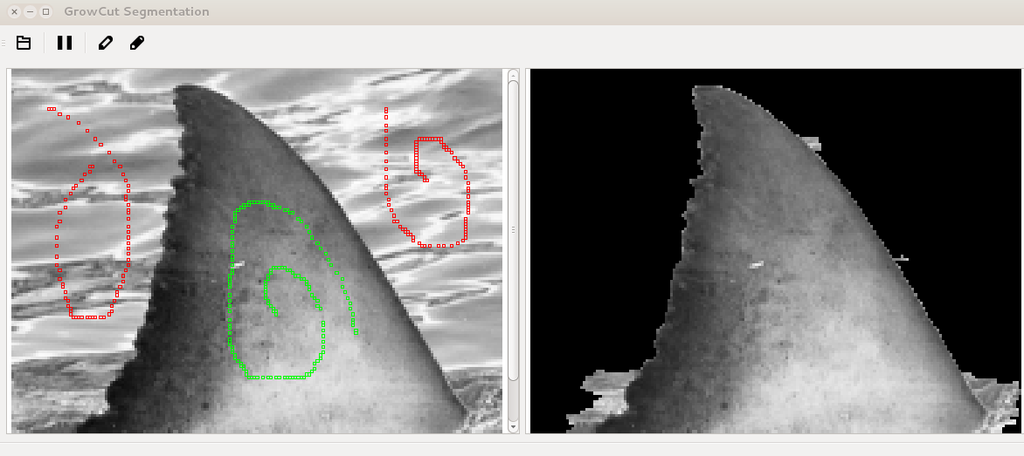
\includegraphics[width=4in, height=1.8in]{haaim}
 \caption{The effect of the modified algorithm}
 \label{fin}
\end{figure}

\noindent It can clearly be seen that the modified version gives better results around the edges, which is essential in the case of the shark fin images.  

\subsection{Random Walker}
The basic method, as
described in \cite{rw} and \cite{rw1}, is as follows.  The user labels a few
pixels as foreground or background for example.  This is then called the seeds. 
A random walker is then released from each of the unlabelled pixels. 
Thereafter, the probability that a certain pixel's random walker first arrives
at a seed with a label, is computed.  In other words, if the user labels $n$
pixels, each with a different label, then the probability that the random walker
leaving the pixel will first arrive at a certain labelled pixel, must be
computed.  The latter is done by modelling the image as a weighted graph, where
the weight of an edge reflects the similarity(intensity values) between pixels,
and solving a system of linear equations.  The pixel is then assigned the label
of the seed for which it is most likely to reach.  The process is repeated until
each pixel is assigned a specific label. 


\subsection{Watershed}
One of the first algorithms tested was the classic watershed algorithm, as
implemented in \cite{scikit}.  The algorithm starts with user-defined markers,
called seed points, which can be viewed as little holes in the image, whereafter
pixel values are treated as a topography/landscape.  The algorithm then floods
basins from the user-defined markers until basins which attribute to different
markers meet at watershed lines.  In this case marker positions are chosen as
the local maxima of the image.  Thereafter the segmentation is done on the
gradient image.  The result of the watershed algorithm applied to a shark fin
image is shown below.

\begin{figure}[H]
\centering
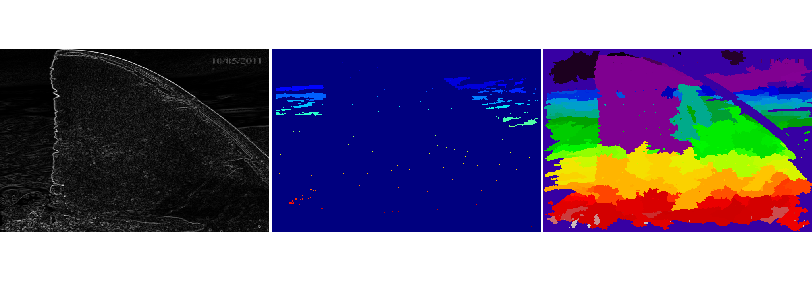
\includegraphics[width=4in,height=2in]{watershed.png} 
\label{fig1}
\caption{Result using the watershed algorithm}
\end{figure}

\noindent The first image shows the gradient image of the original shark fin
image.  The second image shows the pixels that are identified as a local maxima.
 The third image shows how the basins flooded until watershed lines are reached.
 Putting the correct segments together, which will require a lot of hard work,
an effective segmentation can be done.

\section{Results}
\subsection{}

\subsection{}


\section{Conclusions}
\subsection{}

\subsection{}

\subsection{Future work}


\newpage
\bibliography{final}

\end{document}